\section*{Methodology}
\label{sec:methodology}
\subsection*{Methodology overview}
The overview structure of UML diagram is shown in Figure \ref{fig:uml_diagram}.
\begin{figure}[htbp]
    % define the figure title
    \centering
    \includegraphics[width=0.5\textwidth]{figures/uml.png}
    \caption{UML diagram of the methodology: 
    The class: ontology and JSON converter are used to construct the initial ontology framework and store it in the graph database. 
    The ontology enrichment frame are used to identify potential object properties and entities from multimodal data sources, and enrich the data properties of the ontology. The class Query Module are responsible for Question and Answering system and report generation.}
    \label{fig:uml_diagram}
\end{figure}


Our system consists of three components: 
\begin{enumerate}
    \item \textbf{Ontology Framework Construction:}
    
    % We do not rely on large language models (LLMs) to construct the ontology from scratch. 
    % Instead, we create a predefined ontology that defines the domain and ranges of building renovation activities, object properties, 
    % and data properties. This ontology is converted into JSON format and stored in graph databases.
    At the beginning, we construct a predefined ontology regulating the domain and range of classes, object properties, and data properties for safety management in renovation activities.
    The predefined ontology is converted to JSON format and stored in a graph database. 
    
    \item \textbf{Data-Driven Ontology Construction:}
    Data-driven methods are employed to enrich the predefined ontology in two ways:
    \begin{enumerate}
        \item We use LLMs to extract potential object properties and entities from multimodal data sources. These are converted into RDF triples and stored directly in the graph database.
        \item Statistical analysis is performed on the extracted data to enrich the data properties of the ontology. The enriched attributes are then stored in the graph database.
    \end{enumerate}
    \item \textbf{Knowledge Inference:}
    A Retrieval-Augmented Generation (RAG) based method is used to perform knowledge inference and 
    generate reports for safety management in renovation activities. 
    Building Information Modeling (BIM) components are mapped to the ontology through anaphora resolution, 
    and the RAG model interacts with the graph database to generate safety management reports.
\end{enumerate}
\subsection*{Ontology Framework Construction}
\label{sec:ontology_coarse}
% list the standford seven steps for ontology construction
% point out the domain and range of ontology classes and properties are reused from existing ontology
% we use llm only to enrich the ontology from step 4, that is to extract potential object properties and entities
% identify ontology instances and properties, we will not involve in the creation of new classes and define the hierarchy of classes, 
% which is very professional and have high risks, since reliability is not gurananteed, and it is possible to introduce bias
\subsubsection{Ontology Construction}
According to the Stanford seven steps for ontology construction \cite[]{noy2001ontology}, 
the ontology construction process consists of seven steps: \textbf{1.} Define the domain and scope of the ontology, 
\textbf{2.} Consider reusing existing ontologies, 
\textbf{3.} Enumerate important terms in the ontology, 
\textbf{4.} Define the classes and the class hierarchy, 
\textbf{5.} Define the properties of classes, 
\textbf{6.} Define the facets of properties, and
\textbf{7.} Create instances of classes and properties.

Based on literatures, we create a predefined ontology that defines the domain and range of ontology classes and properties for safety management in renovation activities.
The initial ontology framework defines the domain and range of ontology classes and properties. Based on the listed entities and types of relations,
LLMs can extract potential object properties and entities from multimodal data sources to enrich the ontology. 
We also reuse the properties and instances of existing ontologies. The knowledge reasoning is performed on Protégé using semantic web rule language (SWRL) and knowledge reasoning engines like Jena or JESS.
The basic ontology structure is show in Figure \ref{fig:ontology_structure}.
\begin{figure}[htbp]
    % define the figure title
    \label{fig:ontology_structure}
    \centering 
    \includegraphics[width=0.5\textwidth]{figures/ontology.png}
    \caption{Ontology structure}
\end{figure}

% define the pseudo code of ontology conversion here
\subsubsection{Ontology format conversion}
Since the owl format mainly used by Protégé only, for the convenience and speed of data storage and retrieval, we convert the ontology to JSON format and store it in the graph database.
The conversion prcess follows the following princples:
\begin{enumerate}
    \item All the relations can be represented as a triplets, in the format \((O,P,S)\), where the \(O\) is the object, \(P\) is the property, and \(S\) is the subject.
    The triplets are stored in graph databases. The object and subject are two nodes, and the property is the edge connecting the two nodes.
    The data properties for each class are stored as attributes of the node in graph databases. The hierarchy of classes is stored as the parent-child relationship in the graph database.
    \item The children of classes should inherit the properties of their parent classes.
    \item There should be no two same nodes in the graph database.
\end{enumerate}
Following the above principles, we convert the ontology to JSON format and store it in the graph database. 

The conversion process can be recursively conducted on the ontology classes and properties. Since the classes and properties in owl is stored hierarchically,
we first extract the direct properties of the class and then add the properties of the parent class to current class. 
We store the properties as a key-value pair in the JSON format.
 Then, we recursively call the function to convert the children of the class until there are no children class left.
The pseudo code of the owl2json is shown in Algorithm \ref{alg:ontology2json}.
\raggedright
\begin{algorithm}
    \begin{algorithmic}[1]
        \label{alg:ontology2json}
        \Require $ontology$
        \Ensure $json\_ontology$
        \State $json\_ontology \leftarrow \{\}$ 
        \Function{ontology2json}{$ontology,json\_ontology$}
            \For{$class$ in $ontology$}
                \State $json\_ontology[class] \leftarrow \{\}$
                \For{$property$ in $class$}
                    \State $json\_ontology[class][property] \leftarrow \{\}$
                    \For{$value$ in $property$}
                        \State $json\_ontology[class][property].append(value)$
                    \EndFor
                \EndFor
            \EndFor
            \Return $json\_ontology$
        \EndFunction
        % \textbf{Function} $ontology2json(ontologyClass, ParentProperties, JsonFile)$
        %     \FOR{$property$ in $ontologyClass.properties$}
        %         \STATE $JsonFile[ontologyClass][property] \leftarrow ontologyClass.property$
        %         \STATE $JsonFile[ontologyClass][property].append(ParentPropertie[property])$
        %         \STATE $JsonFile[ontologyClass][property] \leftarrow ontologyClass.property$
        %         \STATE $JsonFile[ontologyClass][property].parentParentPropertie.parentName$
        %     \ENDFOR 
        %     \FOR{$child$ in $ontologyClass.children$}
        %         \STATE ontology2json($child, JsonFile[ontologyClass][property], JsonFile$)
        %     \ENDFOR
        %     \textbf{return} $JsonFile$   
        % \Procedure{ontology2json}{$ontology$}
        %     \FOR{$class$ in $ontology$}
        %         \STATE $json\_ontology[class] \leftarrow \{\}$
        %         \FOR{$property$ in $class$}
        %             \STATE $json\_ontology[class][property] \leftarrow \{\}$
        %             \FOR{$value$ in $property$}
        %                 \STATE $json\_ontology[class][property].append(value)$
        %             \ENDFOR
        %         \ENDFOR
        %     \ENDFOR
        %     \RETURN $json\_ontology$
        % \EndProcedure


        \For{$class$ in $ontology$}
            \State $json\_ontology[class] \leftarrow \{\}$
            \For{$property$ in $class$}
                \State $json\_ontology[class][property].append(property) \leftarrow \{\}$   
            \EndFor
            %\State ontology2json($class, json\_ontology[class][property], json\_ontology$)
            % call the function here
            \State $json\_ontology \leftarrow \Call{ontology2json}{class,json\_ontology}$
        \EndFor
        % add comment here in pseudo code


    \end{algorithmic}
\end{algorithm}
After we convert the ontology to JSON format, we store it in the graph database directly using the graph database API and merge the repeatitive nodes in the graph database.
Compare the XML format of the Graph database storation and JSON format of ontology,
 the JSON format is more readable and easy to store and retrieve. 
 Comparing the time to retrieve properties of a class, the JSON format is also faster than XML format in python.
 The detailed comparison is shown in Table % \ref{tab:format_comparison}.


\subsection*{Data-Driven Ontology Construction}
\label{sec:ontology_fining}
In this step we will apply the LLMs to enrich existing ontology. 
Due to the limitation of data, we only design LLM to enrich ontology in two aspects, \ref{tab:ontology_enrichment} :
\begin{table}[htbp]
    \centering
    \label{tab:ontology_enrichment}
    \caption{LLM based ontology enrichment}
    % make table alignment with text
    
    \begin{tabular}{ccc}
        \hline
        \textbf{Domain} & \textbf{Type of Properties} & \textbf{Input format} \\
        \hline
        Risk Frequency  &  Data Property              &  image               \\
        Related Regulation & Object Property           &  text document        \\
        \hline

    \end{tabular}
\end{table}
\subsubsection{Risk Frequency}
The risk frequency is a data property that describes the frequency of risks in renovation activities. 
Current ontology only defines the potential risks related to renovation activities, 
but all kinds of risks share the same weight in the ontology.
We use LLMs to extract the risk frequency from related image from related image database.
The enrichment proces follows the following steps:
\begin{enumerate}
    \item \textbf{Define the range of risks: } \\
    As all possible risks are defined related to renovation activities are all defined in the ontology, 
    we make the LLMs to conduct semantic analysis on the images related to targeted activites. 
    \item \textbf{LLM prompt Tuning: } \\
    We select few images for prompt tuning to make the response of the LLMs more accurate and reliable. 
    The process of prompt tuning is as shown in 


    For stable experiment results, we set the temperature of the LLMs to be 0.1,
     since the higher temperature may introduce randomness to the results, which will affect the reliability of the results.
    \item \textbf{Extract the risk frequency: } \\
    We count the identified risks' frequency in the images and store the frequency as the data property of the ontology.
    If the risk is not related to the renovation activities, we will add the relation to the ontology and write to the graph database.
\end{enumerate}

We display the workflow of the risk frequency extraction in Figure \ref{fig:risk_frequency_workflow}. and samples of risk frequency enrichment in Table \ref{tab:risk_frequency_sample}.
After we store the data in graph database, we can query the frequency of all identified risks related to the renovation activities, see figure \ref{fig:risk_frequency_query}.
\begin{figure}
    \label{fig:risk_frequency_query}
    \centering
    \includegraphics[width=0.5\textwidth]{figures/graph_frequency_query.png}
    \caption{Risk frequency query in graph database: The risk frequency attribute on the risk node indicate the class of risk frequency in related renovation activities.
     The higher number indicates the higher frequency of the risk in the renovation activities.}
\end{figure}

\begin{figure}
    \label{fig:risk_frequency_workflow}
    \centering
    \includegraphics[width=0.5\textwidth]{figures/Data properties enrichment.png.png}
    \caption{Risk frequency extraction Workflow}
\end{figure}
% Here is a sample for activity risk frequency extraction:
\begin{table*}[htbp]
    \centering
    \label{tab:risk_frequency_sample}
    
    \begin{tabularx}{\textwidth}{ccX}
        \hline
        % \multicolumn{3}{c}{Prompt setting} \\
        % \hline
        % %left align the text
        % \multicolumn{3}{l}{Identify risks appear in the following image. The scope of risks are: \textless risks range \textgreater } \\
        % \multicolumn{3}{l}{only return the name of the risks that are present in the images,} \\
        % \multicolumn{3}{l}{the format should be JSON. The outputs should be organized in} \\
        % \multicolumn{3}{l}{the format of risks:[risk1,risk2,risk3]} \\
        % \hline
        \textbf{Activity} & \textbf{Image} & \textbf{Identified Risks} \\
        \hline
        Ductwork\_removal & 
        \raisebox{-\totalheight}{\includegraphics[width=0.3\textwidth]{figures/remove-hvac.jpeg}} 
        & Working\_at\_Height, Falling\_Objects,Slips\_Trips\_and\_Falls, Dust\_and\_Debris \\
        \hline
        Structural\_related & 
       \raisebox{-\totalheight}{\includegraphics[width=0.3\textwidth]{figures/p.jpeg}} 
        & Working\_at\_Height, Slips\_Trips\_and\_Falls \\
        % \includegraphics[width=0.1\textwidth]{figures/p.jpeg}
        %  & Working_at_Height, Slips_Trips_and_Falls \\
        \hline
        Site\_Clearing & 
        
        \raisebox{-\totalheight}{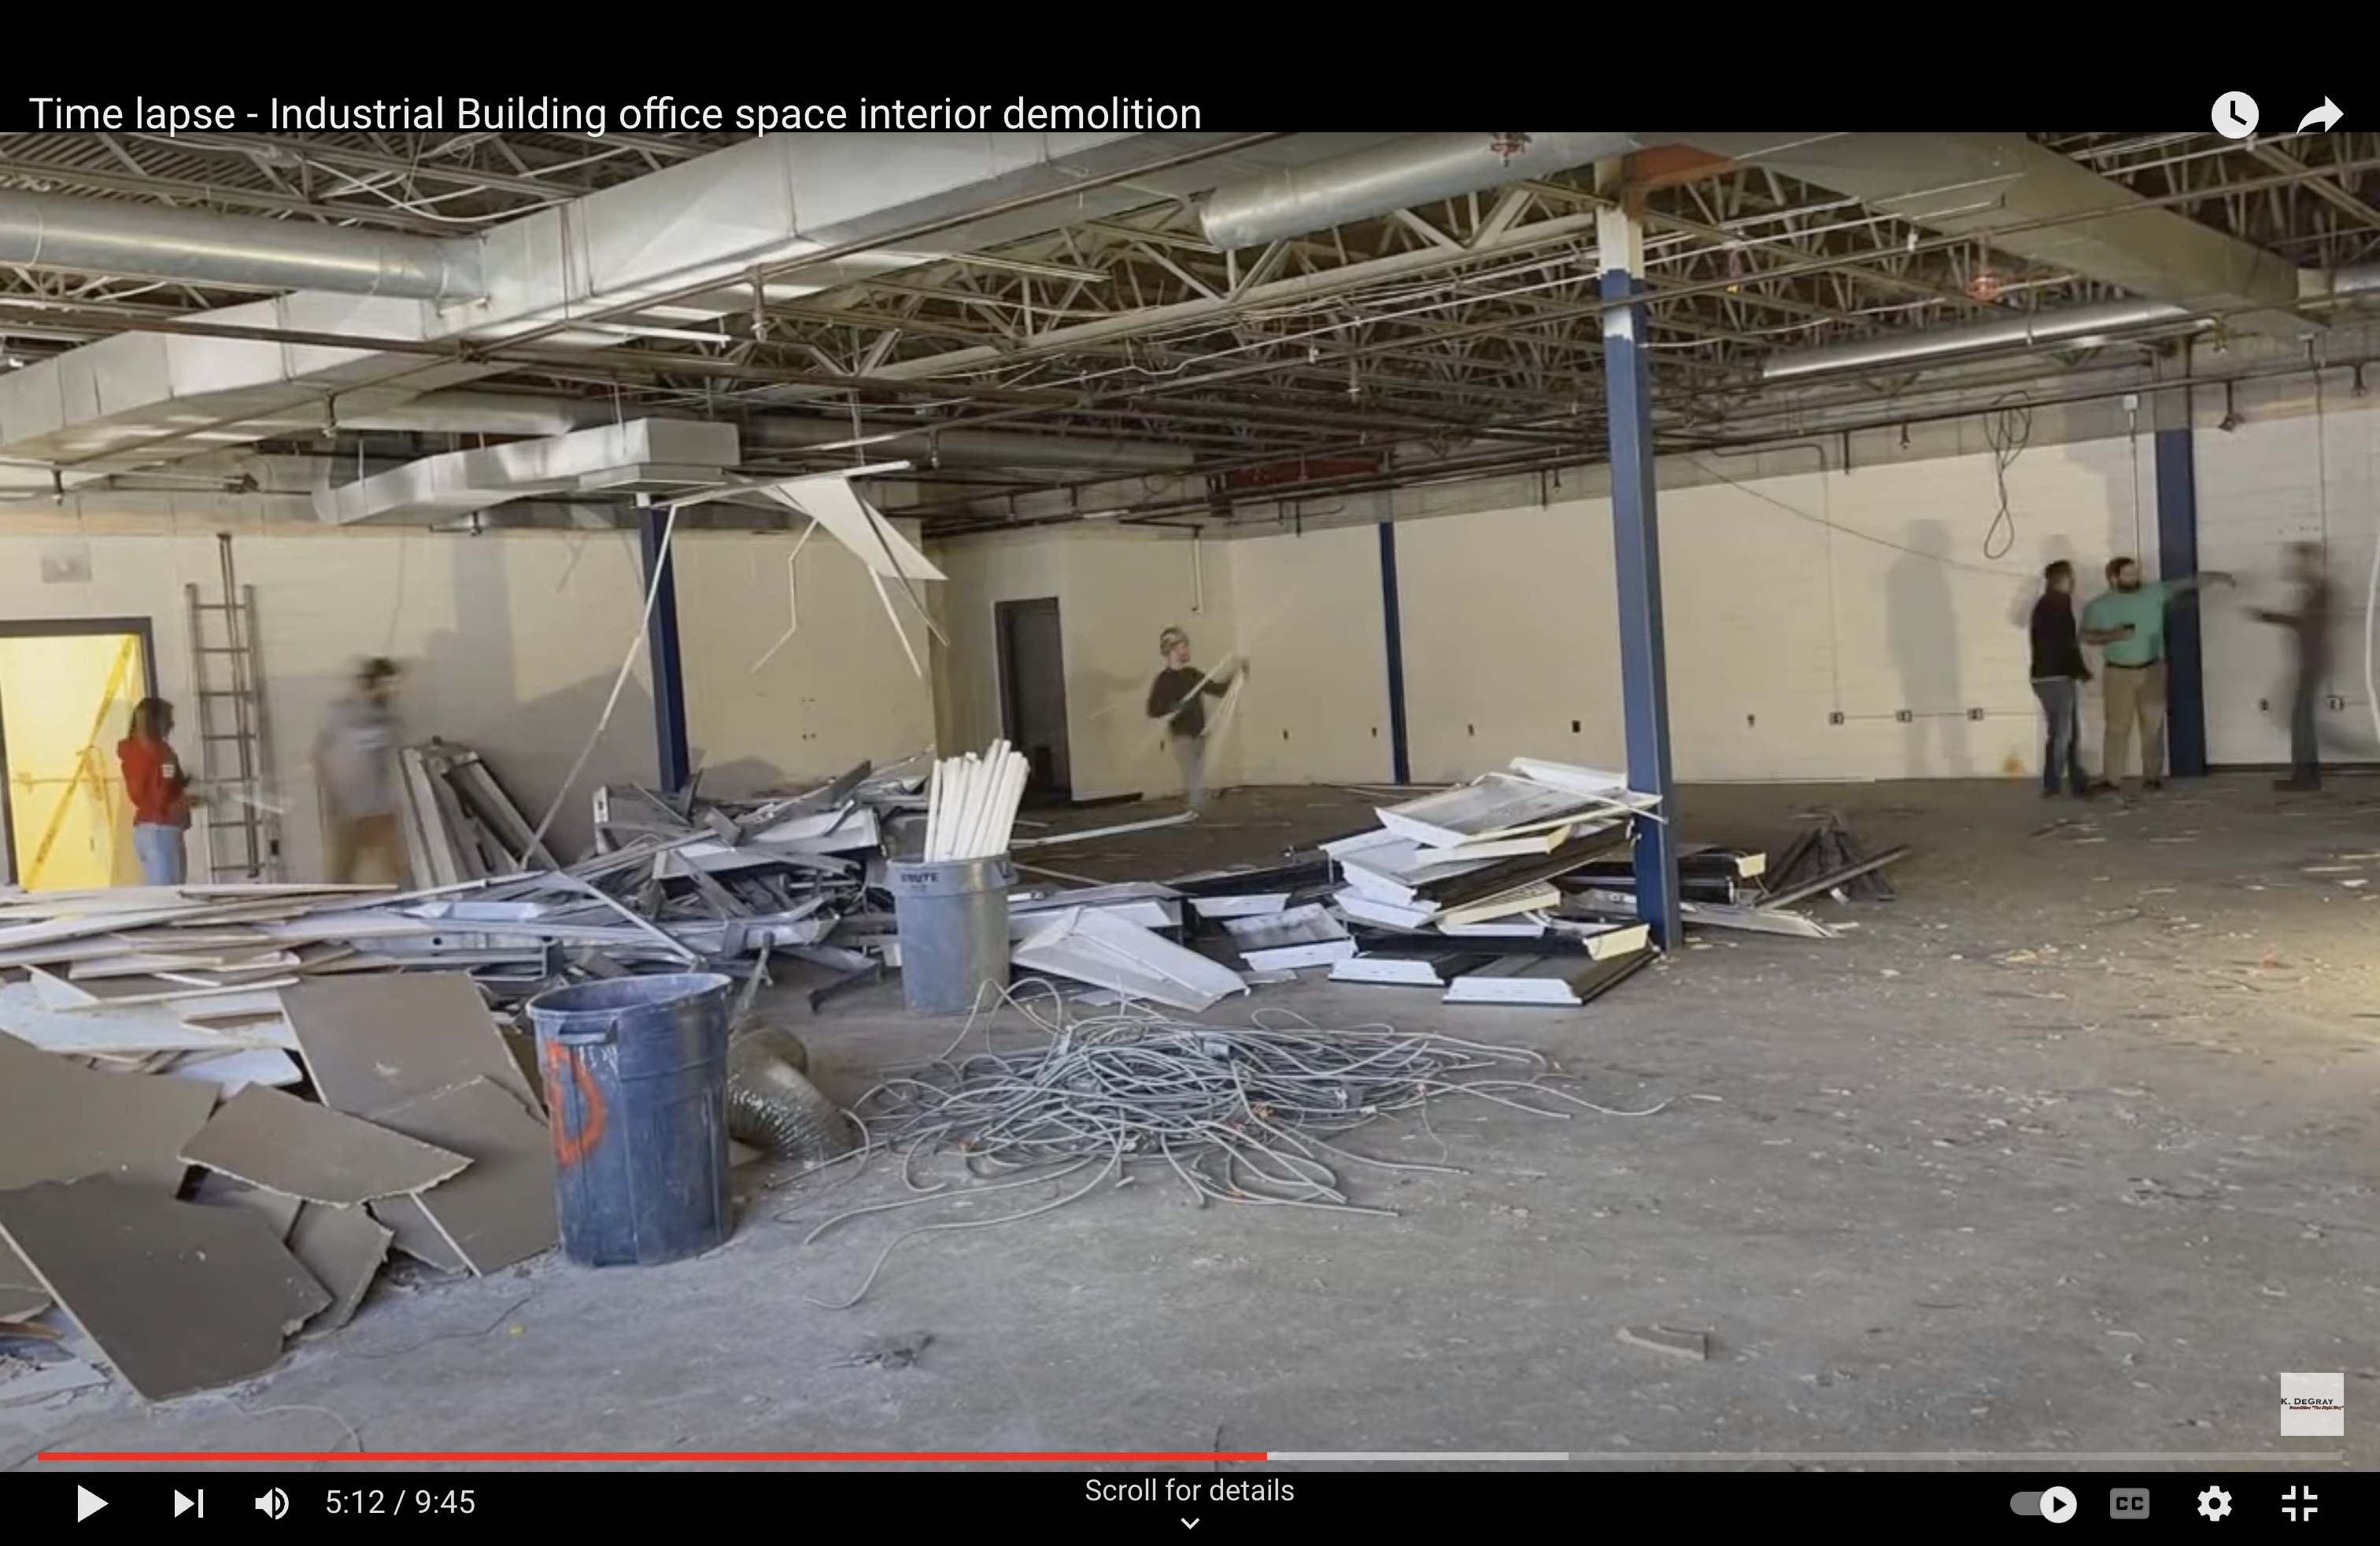
\includegraphics[width=0.3\textwidth]{figures/2024-05-31-5.41.36.png}}
         & Falling\_Objects, Slips\_Trips\_and\_Falls, Dust\_and\_Debris \\
        \hline
    \end{tabularx}
    \caption{Risk frequency enrichment sample}
\end{table*}
\subsubsection*{Regulation Document Processing} 
Applying NLP for information extraction has two branches: traditional methods and deep learning-based methods.
In safe management in building construction area, 
except few study applying machine-learning based methods for information extraction \cite[]{marucci2017classifying},
most of the studies are applying traditional NLP methods for information extraction \cite[]{xu2021extracting,wu2024nlp}. 
Reviewing previous studies, the machine-learning based methods need to train a text classifier based on SVM or naive bayes \cite[]{marucci2017classifying};
the traditional NLP need to setting linguistic rules to extract key word from sentences and have requirement for the quality of the text \cite[]{xu2021extracting,wu2024nlp}.

In our study, we apply Large language model to achieve information extraction from text documents, compared with previous studies,
large language model has two advantages: \textbf{1. High generalization:} 
the large language model can extract information from text documents without setting linguistic rules, only setting the prompt for the model;
\textbf{2. High flexibility:} the large language model can extract information from text documents with different quality, since the model is trained on large corpus of text data.

The process of information extraction is as follow:
\begin{enumerate}
    \item \textbf{Define the range of activities and entities: } \\
    From the graph database we extract the range of all possible activities and entities related to the input regulation documents. 
    \item \textbf{Identify the activities relted to the regulation: } \\
    Identify all possible activities related to the regulation documents
    \item \textbf{Identify the entities related to the activities: } \\
    Given each identified activity, we hope that we can also identify the entities involved in the activities, such as 
    building slabs, ceillings, cranes and so on.
    \item \textbf{LLM prompt Tuning: } \\
    Given the sample of regulation documents we continue to tune the LLM prompt to make the response of the LLMs more accurate and reliable.
    \item \textbf{Extract the related regulation: } \\
    We extract the related activities and entities involve in the activity from regulation document and store the information in the graph database.
\end{enumerate}

The process of related regulation extraction is shown in Figure \ref{fig:related_regulation_workflow}.
\begin{figure}
    \label{fig:related_regulation_workflow}
    \centering
    \includegraphics[width=0.5\textwidth]{figures/text_extraction.png}
    \caption{Regulation Document processing Workflow}
\end{figure}

The regulation document processing results is shown in Table \ref{tab:related_regulation_sample}. %add a footnote that the regulation1,2,3 are in the appendix
And the final output on the graph database is shown in Figure \ref{fig:related_regulation_query}.
\footnote{the document of regulation1,2,3 are in the appendix}

\begin{table}
    \centering
    \label{tab:related_regulation_sample}
    \begin{tabularx}{0.5\textwidth}{cX}
        % \hline 
        % \multicolumn{2}{c}{Prompt setting} \\
        % \multicolumn{2}{c}{Identify the activities among:  \textless exists\_activities \textgreater regulated by the given regulation
        % and the entities involved in the regulation among: \textless exists\_entities \textgreater
        % the resonpose should be divided according to the activities and its entities
        % only return the name of the entities and activities the regulation applicable to, and retun the format should be json. in the format of 
        % \textless activities1:[entities1,entities2,...],activities2:[entities1,entities2,...],...\textgreater, all the terms of entities and activities should be appeared in the database}
        \hline
        \textbf{Regulation Document} & \textbf{Identified Activity:[entities]}  \\
        \hline
        regulation1 & Floor\_Slab\_removal:[Concrete\_Foundation\_Slab], \newline Reinforcing\_Bars\_removal:[Reinforcing\_Bars]  \\
        \hline
        regulation2 & Demolition\_Activity:[Mechanical\_Equipment,Floor, \newline Working\_Surfaces,Cranes,Derricks]  \\
        \hline
        regulation3 &  Structural\_demolition:[Nominal\_Breaking\_Strength, Crane\_Boom, Loadline,SwivelType\_Connection, Steel\_Members, Roof\_Cornice] \\
    \end{tabularx}
    % add a footnote that the regulation1,2,3 are in the appendix
    \caption{Related Regulation extraction sample}
\end{table}

\begin{figure}
    \label{fig:related_regulation_query}
    \centering
    \includegraphics[width=0.5\textwidth]{figures/regulation relation.png}
    \caption{Related Regulation query in graph database: The related activities and entities are stored in the graph database.}
\end{figure}

\subsection*{Knowledge Inference}
\label{sec:knowledge_inference}
% define the RAG model
The final step is to build a Question and Answering system and report generation system based on the ontology.
The input will be the question and answer between user and system, and the BIM model of the renovation activities.
The output will be the report of the safety management in renovation activities. 
The report will contains the following information:
\begin{itemize}
   \item \textbf{Activity: } 
   Based on the components of the BIM model and question and answer between user and system,
    the system will identify the activities related to the renovation activities.
    And the system will also list the entities involved in the activities such as building slabs, ceillings, cranes and so on.
    \item \textbf{Risk: }
    Based on the identified activities and entities, the system will identify all the potential risks related to the renovation activities.
    Based on the statistical analysis of the risk frequency, the system will also return the statistical analysis of the risk frequency.
    \item \textbf{Regulation: }
    Based on the activities involved in the building renovation, the system will also return the related regulations
    and also the regualted entities included in the regulated activities. 
\end{itemize}

The whole process of Question and Answering system is decomposed into the following steps:
\begin{enumerate}
    \item \textbf{Mapping BIM components to ontology: } 
    Firstly, we extract all the components of the BIM model, and searching the corresponding entities related to the components,
    which are stored in the graph database.
    \item \textbf{Identify the activities: }
    The range of all possible activities are identified based on recogoized entities from the graph database. 
    Firstly, We use the relation $hasEntity$ to match all possible activities from graph database, including demolition and installation activities. 
    Then, we narrow the range of activities based on the question and answer between user and system. 
    Lastly, we display all the identified activities and entities involved in the renovation, 
    if user agree with the identified activities and entities involving in, we continue to the next step,
    otherwise, we will ask user to make supplement to the identified activities and entities, and repeat the process.
    \item \textbf{Identify the risks and regulation: }
    We return information in three aspects:
    \begin{enumerate}
        \item \textbf{Risk: } 
        We return the risk and the frequency of risk related to the renovation activities.
        \item \textbf{Regualtion: }
        We return the related regulations and entities involved in the regulation.
        \item \textbf{Cases: }
        We return the cases related to the high frequency risks and the related regulations.
    \end{enumerate}

    We make LLM summarize the identified risks and regulations and cases, and generate the report for the safety management in renovation activities.
\end{enumerate}

Compared with traditional ontology-based method that use SPARQL query to obtain knowledge from ontology,
We make LLM to interact with user and system and establish mapping between BIM components and ontology. 
The advantages is that: \textbf{1. Objective: } the LLM can process the querying process objectively and accurately,
excluding the bias introduced by human; \textbf{2. High flexibility: } 
The information is passed to the LLM in the form of prompt, which is more flexible and generalizable than the SPARQL query.
User, especially the non-professional user, can easily interact with the system and obtain the information they need.
The workflow of the knowledge inference is shown in Figure \ref{fig:knowledge_inference_workflow}.
\begin{figure}
    \label{fig:knowledge_inference_workflow}
    \centering
    \includegraphics[width=0.5\textwidth]{figures/qa system.png}
    \caption{Knowledge Inference Workflow}
\end{figure}
\subsection{Summary}
In this section, we propose a methodology for safety management in renovation activities based on ontology and multimodal data sources.
We first construct a predefined ontology that defines the domain and range of ontology classes and properties for safety management in renovation activities.
Then, we apply LLMs to enrich the ontology by extracting potential object properties and entities from multimodal data sources.
We also apply LLMs to extract risk frequency from images and related regulations from text documents.
Finally, we build a Question and Answering system and report generation system based on the ontology to support safety management in renovation activities.
The system can interact with users and BIM models to identify activities, risks, and regulations related to renovation activities.
The system can also generate reports for safety management in renovation activities based on the identified information.
The whole workflow is shown in Figure \ref{fig:methodology_workflow}.
\begin{figure*}[htbp]
    
    \label{fig:methodology_workflow}
    \centering
    \includegraphics[width=\textwidth]{figures/total workflow.png}
    \caption{Methodology Workflow}

\end{figure*}